A utilização da metodologia detalhada no \chapterautorefname~\ref{cap-metodologia} em conjunto com a implementação da proposta definida no \chapterautorefname~\ref{cap-desenvolvimento},  permitiu o desenvolvimento de um robô simulado capaz de explorar um ambiente desconhecido. Neste capítulo, é exposto e discutido os resultados obtidos com a implementação da solução para o problema norteante deste trabalho. 

\section{Modelo Proposto}
O modelo proposto é constituído por três segmentos: i) a simulação; ii) controle lógico e iii) integração dos componentes. Em seguida, são expostos os resultados obtidos no desenvolvimento de cada segmento.

A estrutura física simulada do robô do presente trabalho foi baseado no modelo disponibilizado por \citet{modeloRobo}. O AtmosBot (Figura~\ref{fig:fotoRobo}) apresenta uma base  tridimensional com quatro rodas comuns e um sensor LiDaR acoplados a ela. Ademais, foi incrementado uma estrutura horizontal  tridimensional com bordas arredondadas e altura de 0,6 metros, no intuito de ser utilizada futuramente como suporte para os instrumentos de localização e manipulação de objetos.

\begin{figure}[h]
    \centering
    \caption{Estrutura física do AtmosBot}
    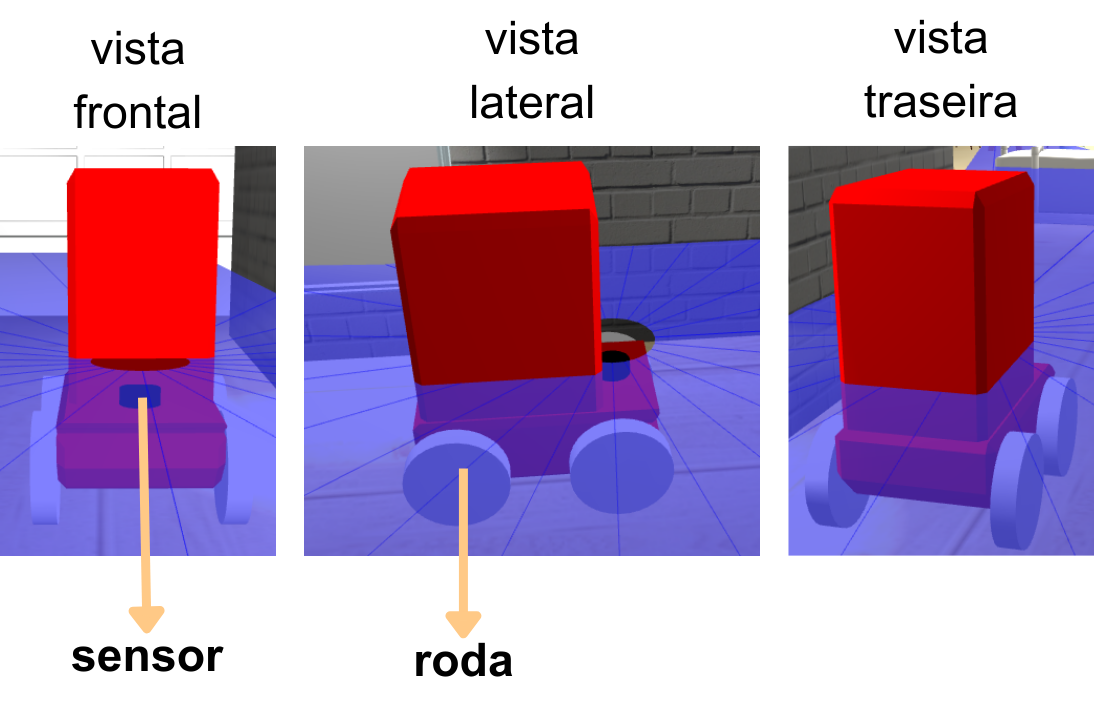
\includegraphics[scale=0.5]{robo.png}
    \caption*{Fonte: Autora (2023).}
    \label{fig:fotoRobo}
\end{figure}

As rodas e o sensor são elementos separados que se integram com a estrutura base do robô a partir das articulações demonstradas na Figura~\ref{fig:roboArticulacoes}. Para as rodas, nos arquivos de descrição de robôs, foi especificado que suas articulações são móveis com o movimento de revolução. Entretanto, para a articulação do sensor, foi definida para se manter estática, a fim de evitar qualquer movimentação indesejada.

\begin{figure}[H]
    \centering
    \caption{Diagrama de articulações do AtmosBot}
    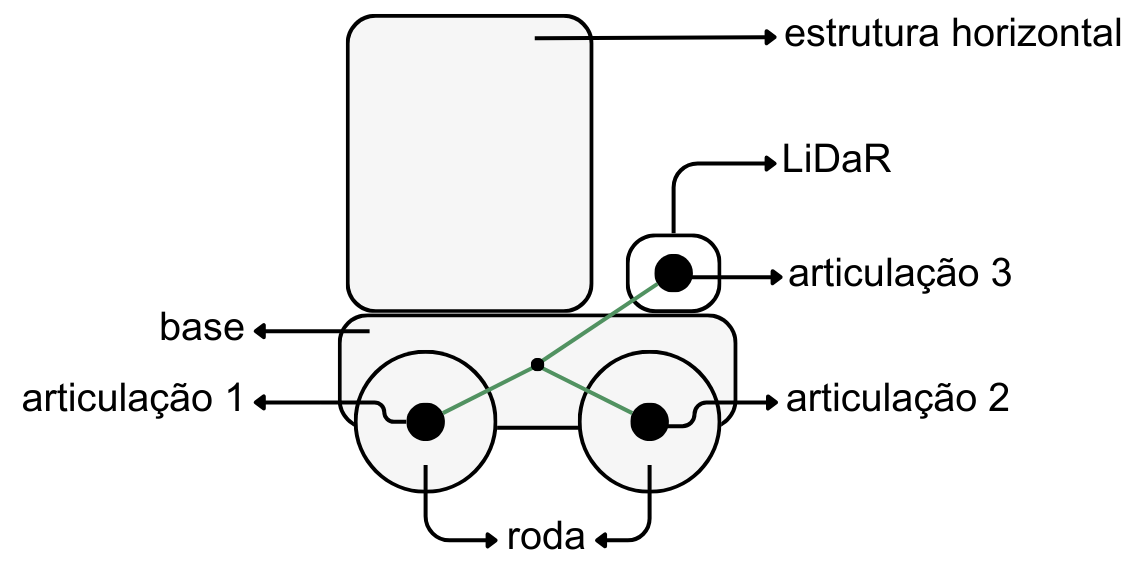
\includegraphics[scale=0.4]{articulacoes.png}
    \caption*{Fonte: Autora (2023).}
    \label{fig:roboArticulacoes}
\end{figure}

O controle lógico do robô está diretamente conectada com a sua navegação autônoma. Os módulos que controlam o robô, para ele se movimentar autonomamente sem colidir com os obstáculos, utilizam as informações do ambiente captadas pelo sensor LiDaR. Na parte superior da Figura~\ref{fig:visaoLidar}, é possível visualizar os feixes de luz do sensor, representados pelas linhas azuis, no simulador Gazebo. Esse sensor atua na horizontal, contendo 24 raios com uma distância de 15 graus entre eles e um alcance de 3,5 metros. Cada feixe capta a distância, em metros, do seu ponto de origem até o obstáculo à sua frente que reflete as ondas óticas. Foi utilizado o valor mínimo entre as distâncias captadas no intervalo de 90 graus em cada extremidade, para identificar os pontos com obstáculos mais próximos nas laterais. Pelo programa RVIZ, na parte inferior da Figura~\ref{fig:visaoLidar}, as capturas do LiDaR são expostas em esferas vermelhas.

\begin{figure}[H]
    \centering
    \caption{Capturas do sensor LiDaR}
    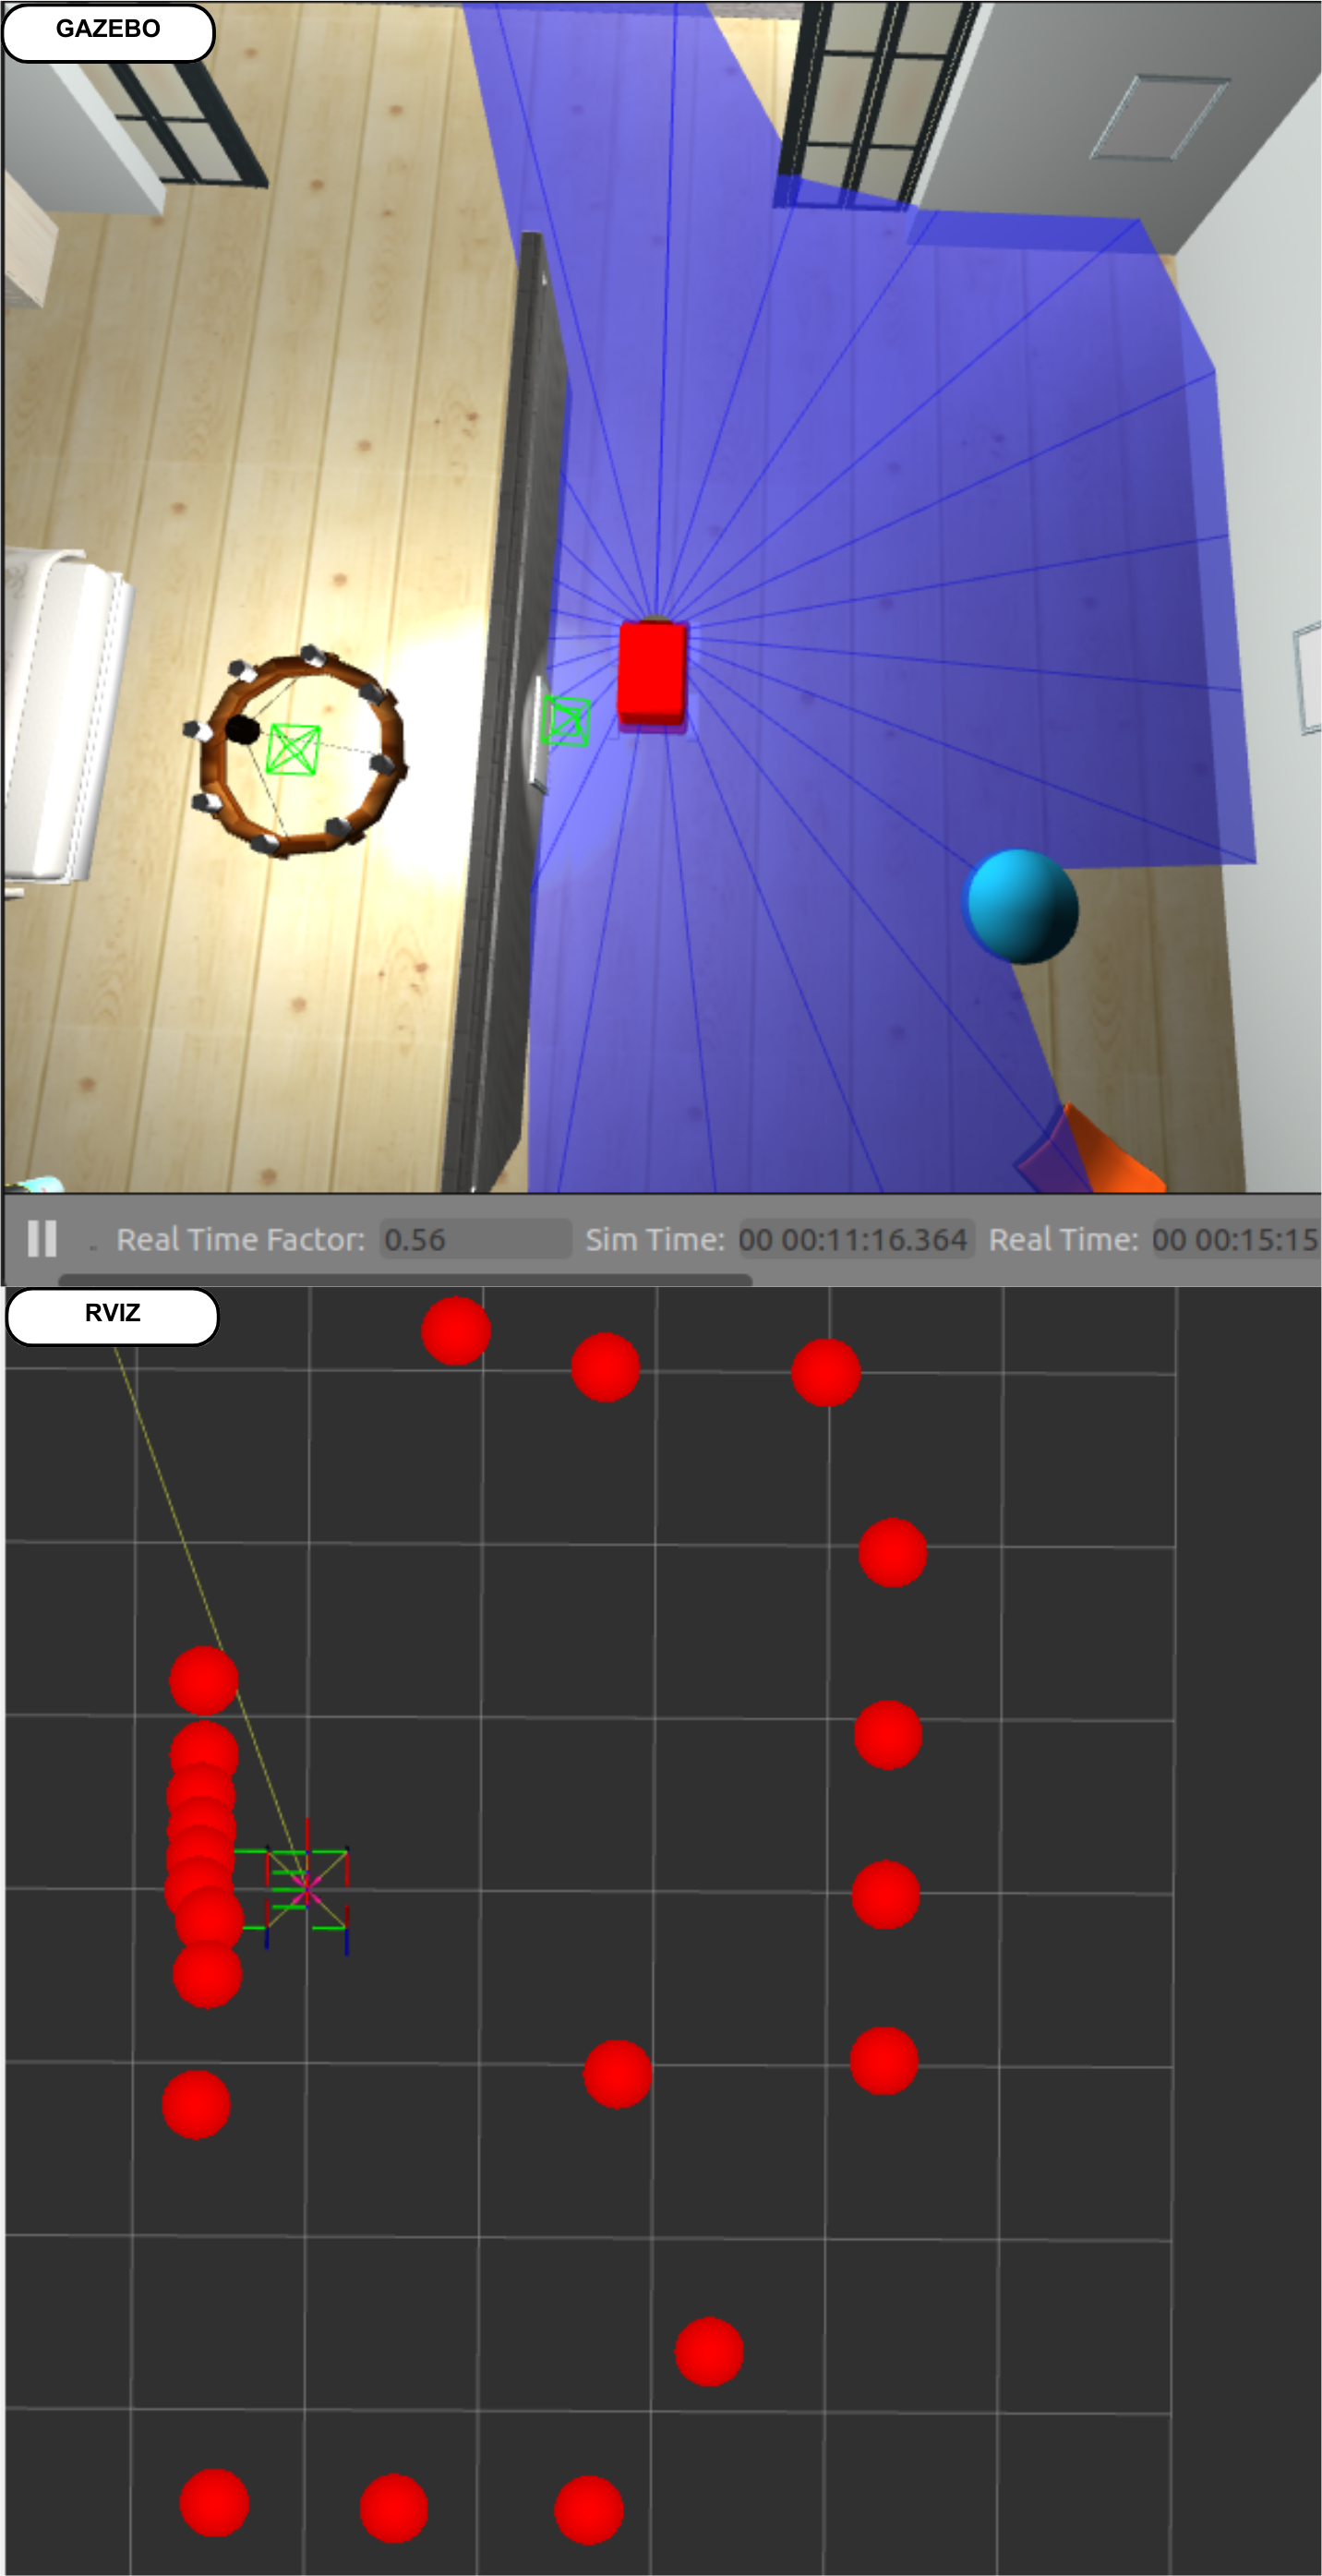
\includegraphics[scale=0.25]{laser.png}
    \caption*{Fonte: Autora (2023).}
    \label{fig:visaoLidar}
\end{figure}

Neste trabalho, o sensor LiDaR permitiu a detecção de obstáculos para que o AtmosBot conseguisse navegar com o mínimo de colisões. Segundo \citet{dpoom}, a câmera RGB com profundidade também é um instrumento muito utilizado para a detecção de obstáculos, podendo ser considerada um recurso mais barato. Entretanto, \citet{navegacaoSlam:2022} identifica que existe um custo maior no processamento das informações de profundidade disponibilizadas por tais câmeras. Por outro lado, como comprovado por \citet{navegacaoSlam:2022}, o sensor LiDaR  alcança o mesmo objetivo de detectar obstáculos durante a navegação do robô de forma satisfatória, com menor custo computacional. Além disso, os resultados obtidos da pesquisa bibliográfica para instrumentos de percepção do ambiente (Figura~\ref{fig:graficoPesquisaPercepcao}) revelam uma maior porcentagem de utilização do sensor LiDaR em trabalhos correlatos. Portanto, visto seu menor custo de processamento, capacidade similar de detecção de obstáculos e alta relevância, é mais coerente e vantajoso utilizar o LiDaR no cenário da problemática deste trabalho. 

Ao longo da exploração do ambiente pelo AtmosBot, o módulo Slam Toolbox cria (e atualiza) um mapa com as informações capturadas pelo LiDaR e pela odometria. Esse mapa é constituído por \textit{pixels} brancos, que correspondem a áreas livres, e pretos, equivalentes aos obstáculos. Pelo programa RVIZ é possível visualizar o mapa sendo criado, como disposto na parte inferior da Figura~\ref{fig:mapaRviz}, conforme os obstáculos presentes na simulação, representada na parte superior da Figura~\ref{fig:mapaRviz}.

\begin{figure}[H]
    \centering
    \caption{Mapa em criação pelo Slam Toolbox}
    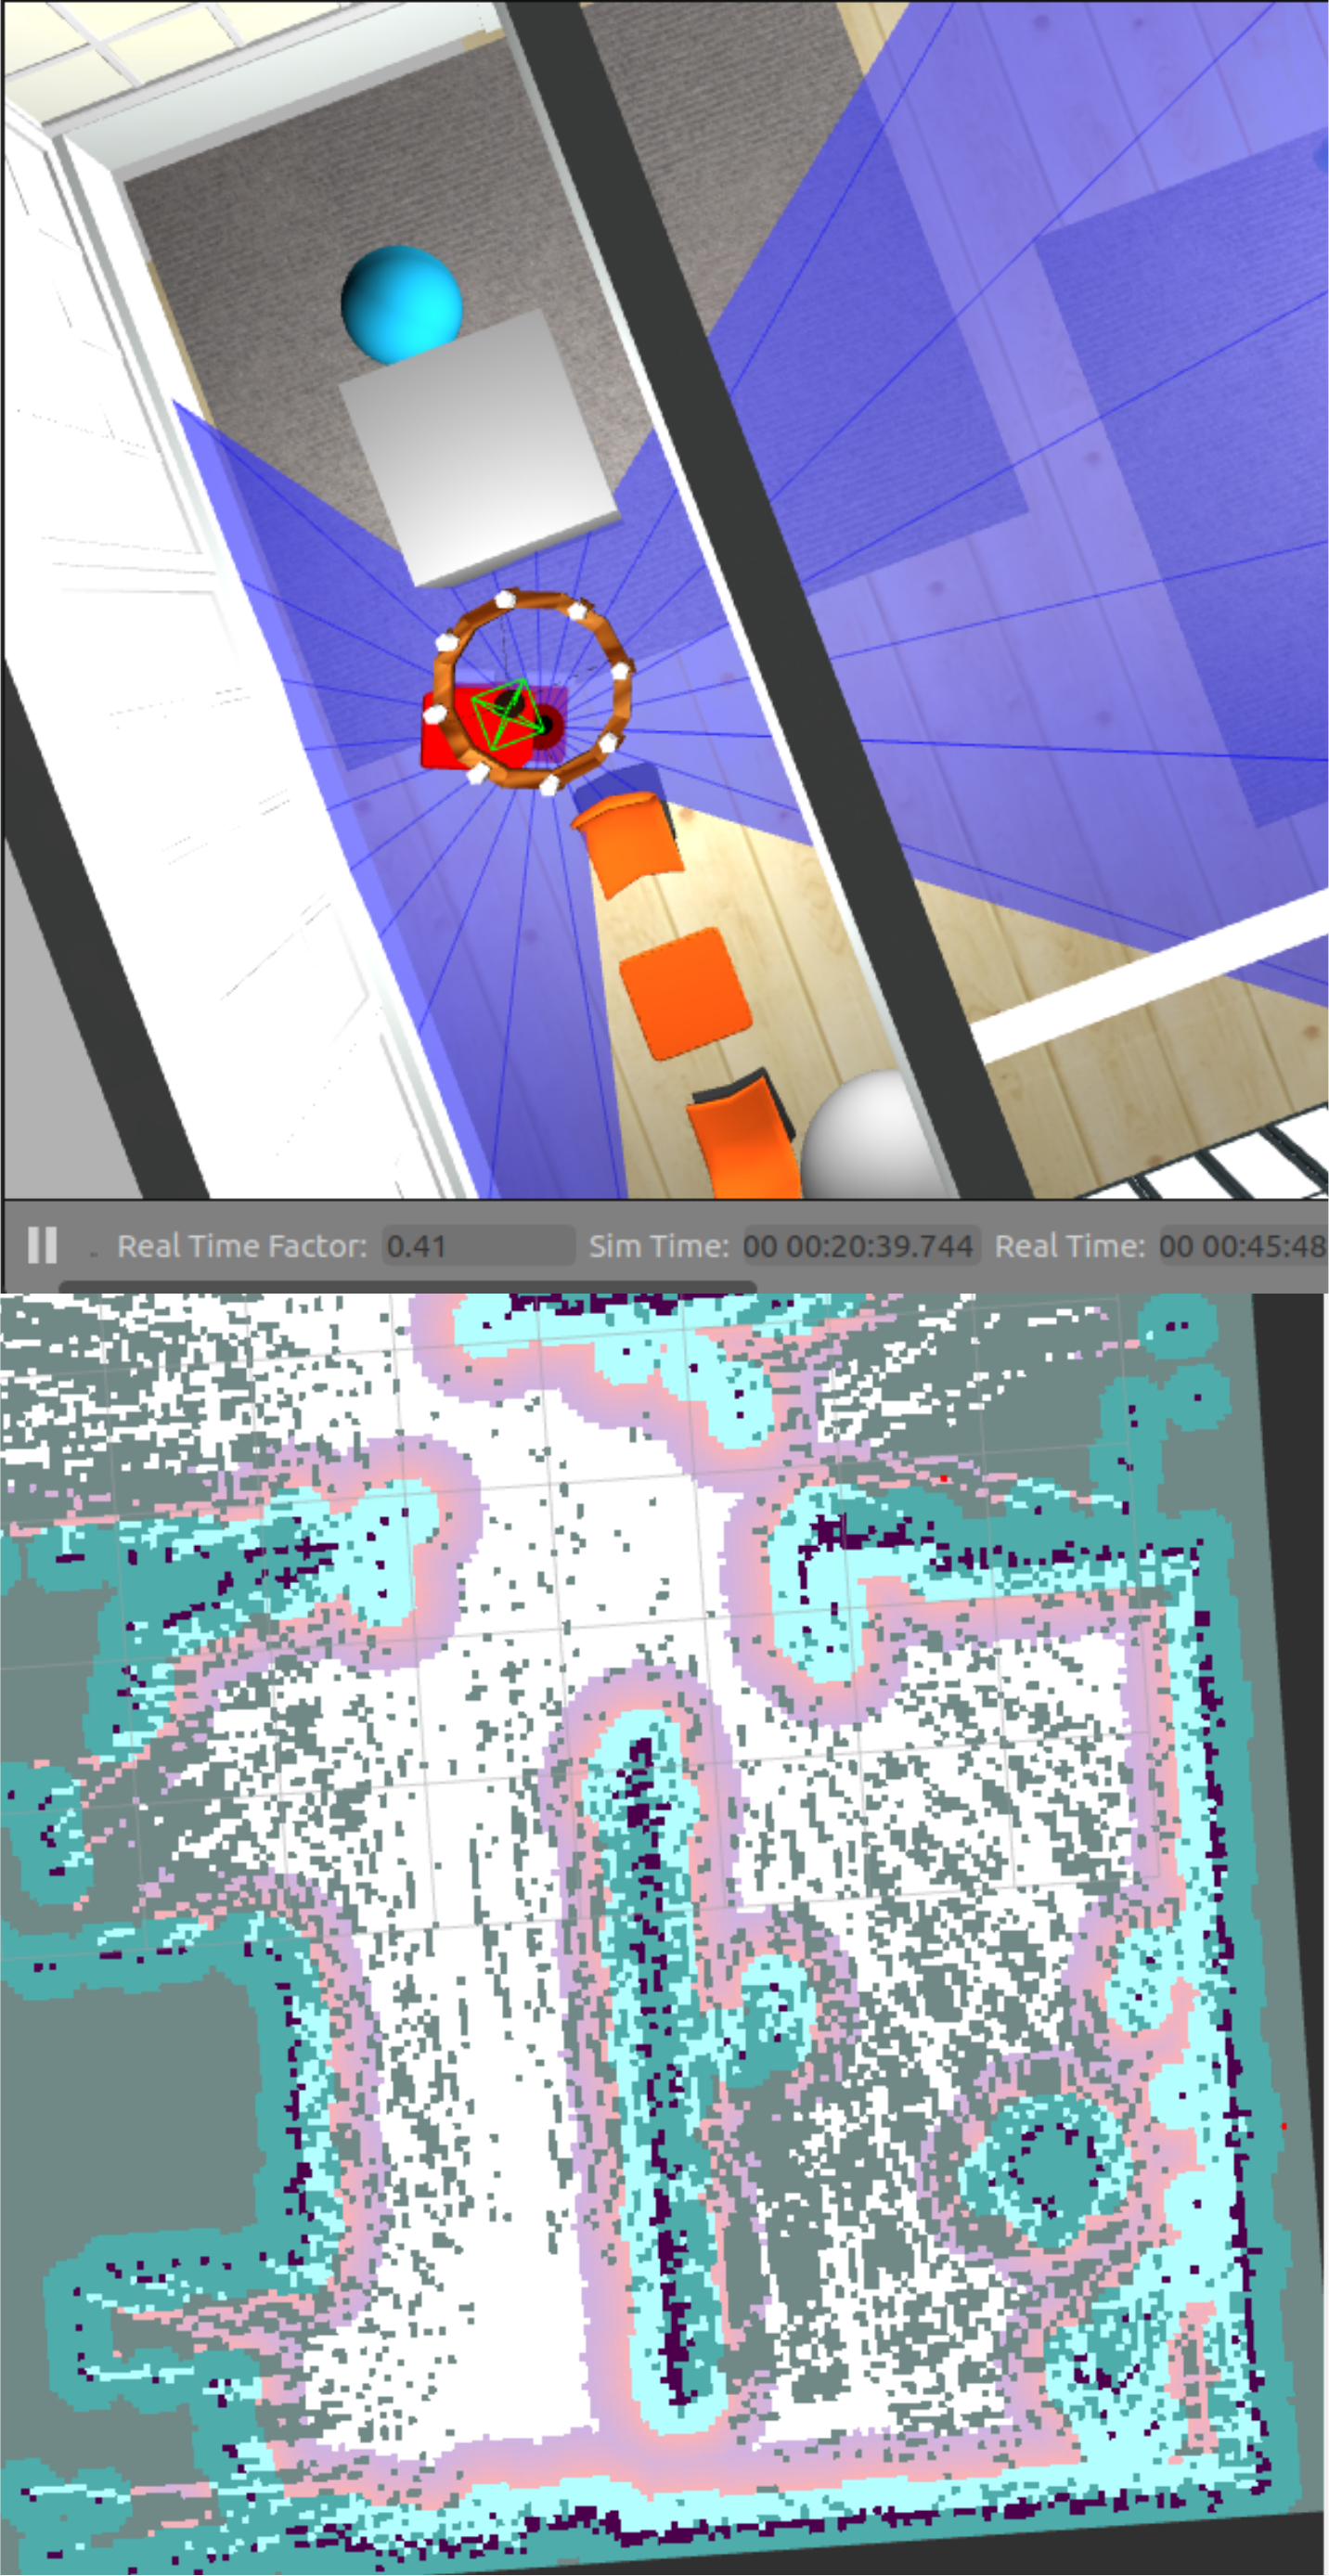
\includegraphics[scale=0.2]{mapRVIZ.png}
    \caption*{Fonte: Autora (2023).}
    \label{fig:mapaRviz}
\end{figure}

No momento de execução, além do mapa de obstáculos e áreas livres, é criado em tempo real um mapa temporário com as áreas de colisão, nomeado como mapa de custos. Nesse formato de mapa, são definidos pesos (custos) para cada área do ambiente, definindo valores maiores para áreas ocupadas por obstáculos e valores intermediários para um raio ao redor dos elementos a serem evitados. Na parte inferior da Figura~\ref{fig:costmap}. estão expostos os obstáculos presentes na simulação (na parte superior da figura). A cor roxa representa uma área perigosa, próxima a um obstáculo. O vermelho indica uma área de colisão com algum elemento do ambiente. Por fim, em azul são representados o centro de massa dos obstáculos.

\begin{figure}[H]
    \centering
    \caption{Mapa de custos temporário}
    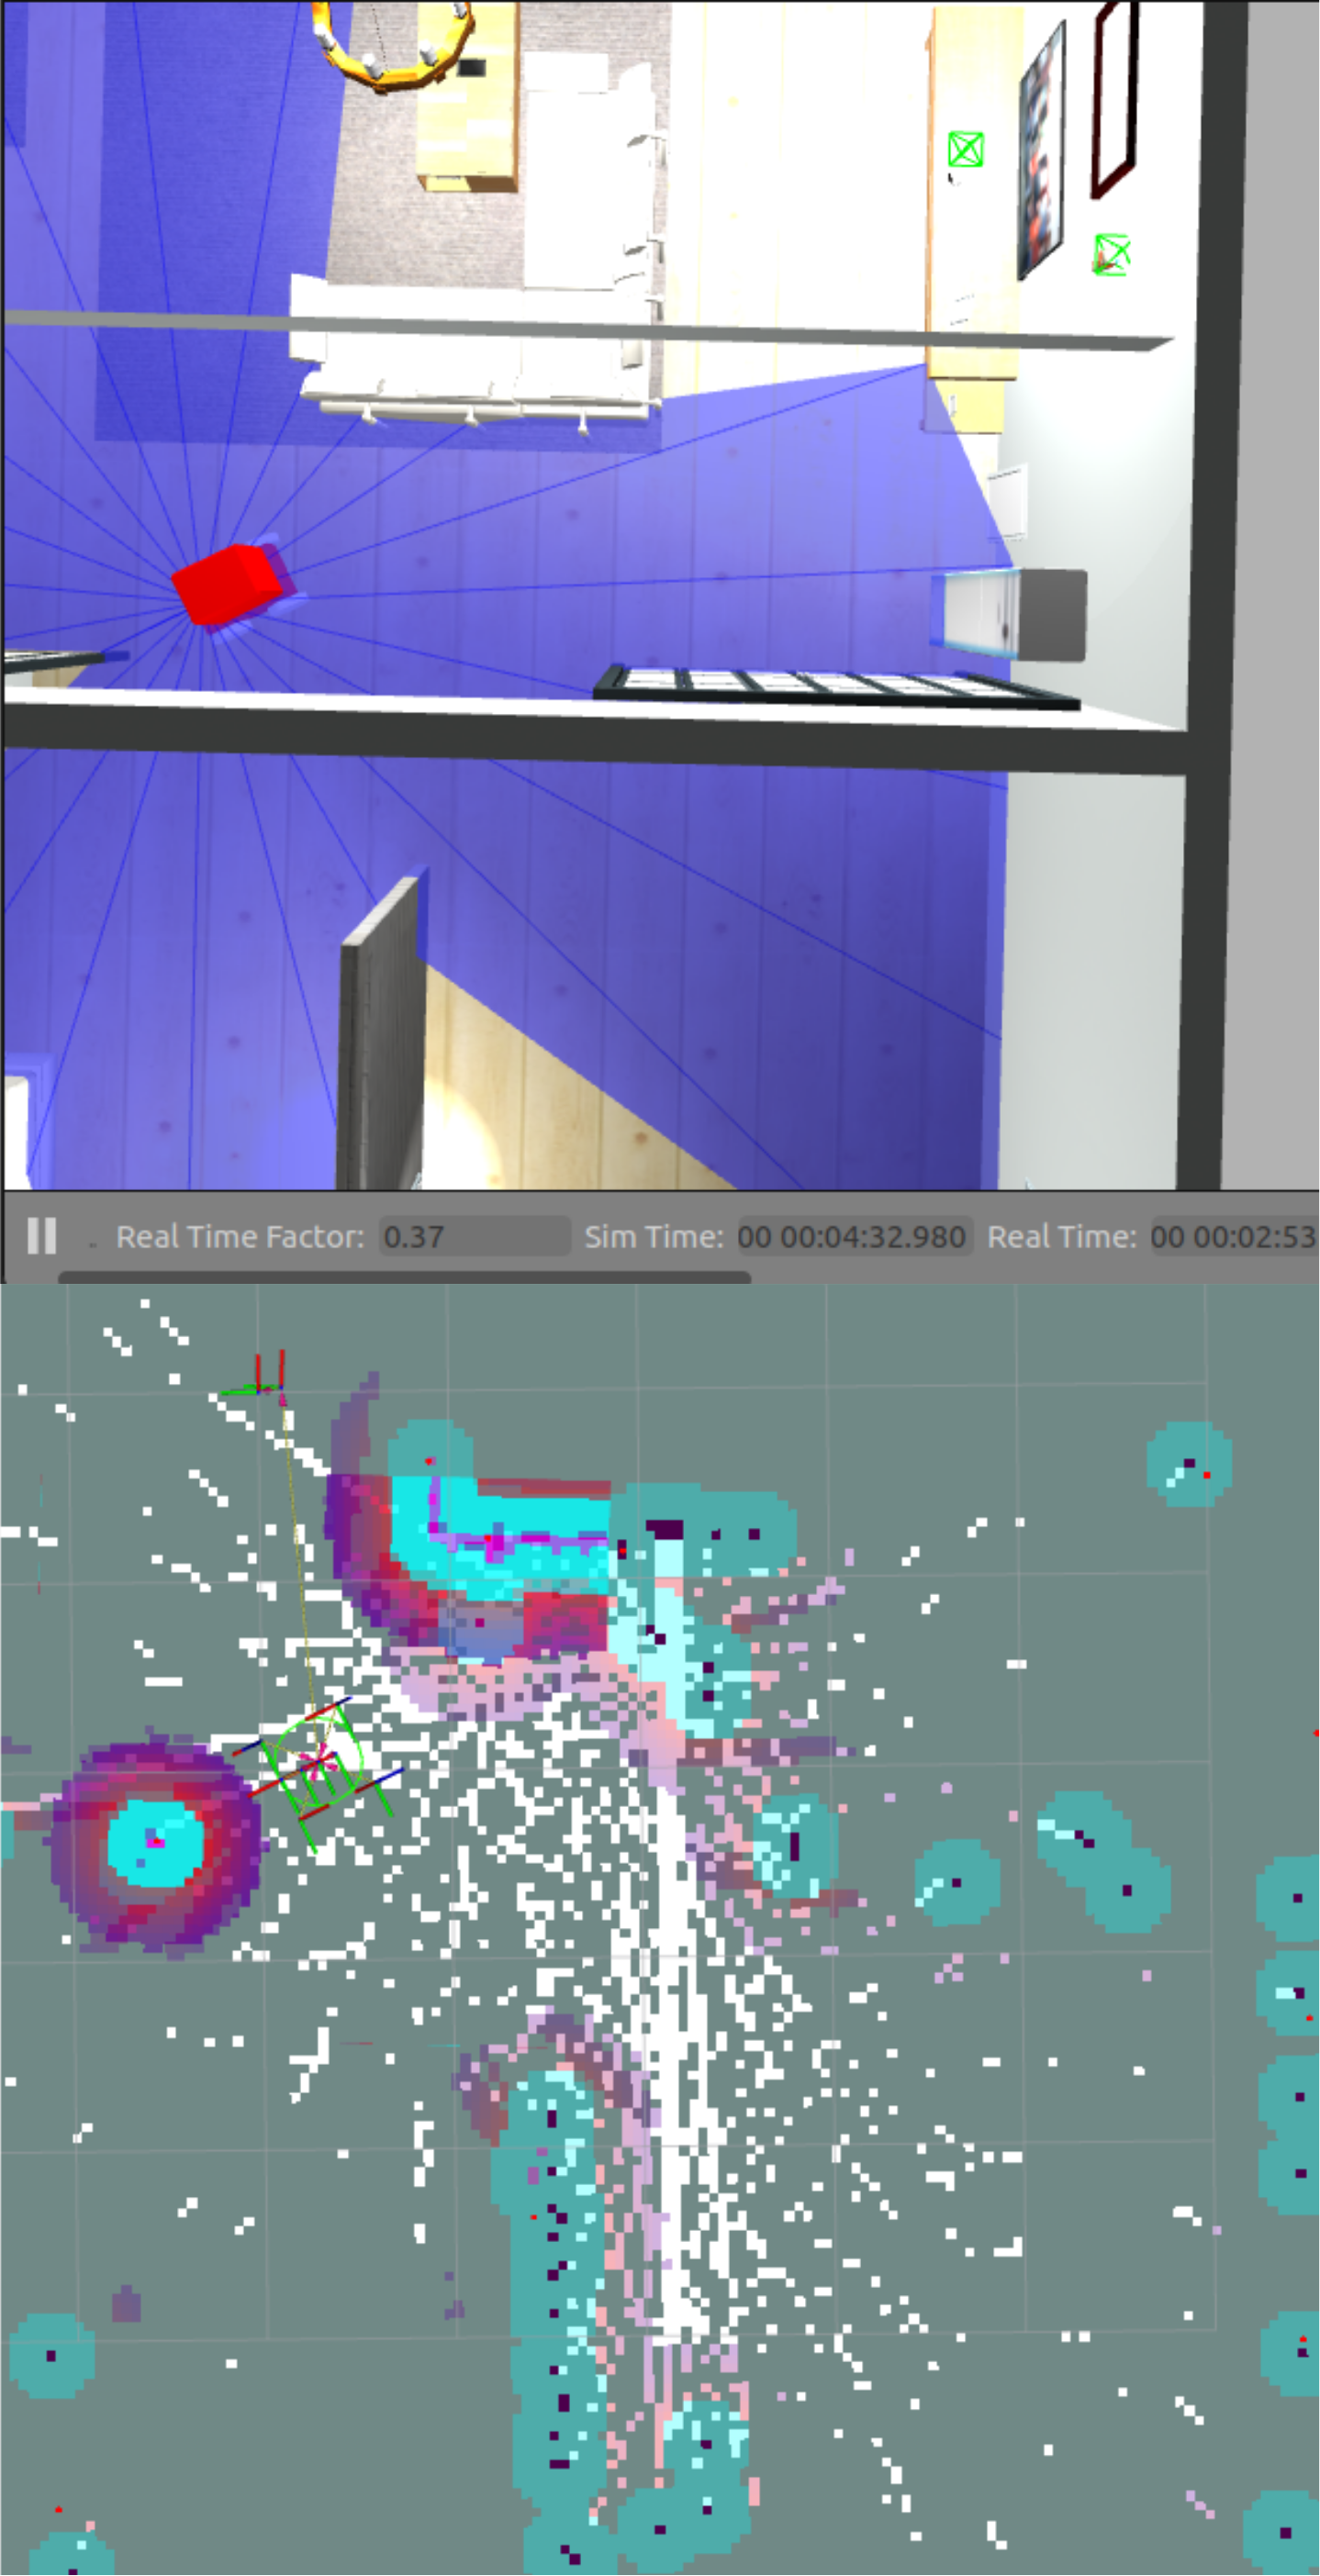
\includegraphics[scale=0.26]{costmap.png}
    \caption*{Fonte: Autora (2023).}
    \label{fig:costmap}
\end{figure}

Com o ambiente completamente, ou parcialmente, explorado, a biblioteca Slam Toolbox permite salvar o mapa de obstáculos, criado com a navegação autônoma, em formato de imagem (Figura~\ref{fig:mapaImagem}) ou serializado. Como o ambiente em que o AtmosBot atua é desconhecido, o seu mapeamento é realizado durante a sua exploração conforme as informações do sensor LiDaR. Em \citet{navegacaoSlam:2022} o ambiente foi mapeado pelo robô controlado remotamente para, em seguida, iniciar sua navegação autônoma com o mapa criado. Essa abordagem resultou em uma divergência de 0,2 metros entre o modelo produzido e a realidade. Assim, para não encontrar essas diferenças, é mais vantajoso mapear o ambiente autonomamente enquanto o robô explora o meio e evitar colisões a partir das capturas do LiDaR. Além disso, como visto, o Slam Toolbox fornece a possibilidade de atualizar o mapa que será utilizado para a localização do robô por outros módulos. 


\begin{figure}[H]
    \centering
    \caption{Imagem do mapa criado pela exploração}
    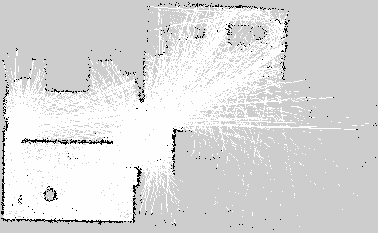
\includegraphics[scale=1]{saved_map.png}
    \caption*{Fonte: Autora (2023).}
    \label{fig:mapaImagem}
\end{figure}


O mapa de áreas livres disponibilizado pelo módulo Slam Toolbox é acessado pela biblioteca Nav2. Com o mapa e a posição atual do robô, é possível identificar a sua localização no ambiente. Pelo programa RVIZ é possível emitir uma instrução para o robô, definindo um ponto de destino. O módulo Nav2 oferece o suporte para realizar a navegação até o objetivo definido de forma autônoma sem colidir com os obstáculos identificados ao longo do caminho. Na Figura~\ref{fig:trajetoriaNav2}, está destacada a trajetória definida para o ponto de destino, representada como uma linha vermelha, conforme o comando inserido no RVIZ.


\begin{figure}[H]
    \centering
    \caption{Trajetória elaborada pelo Nav2}
    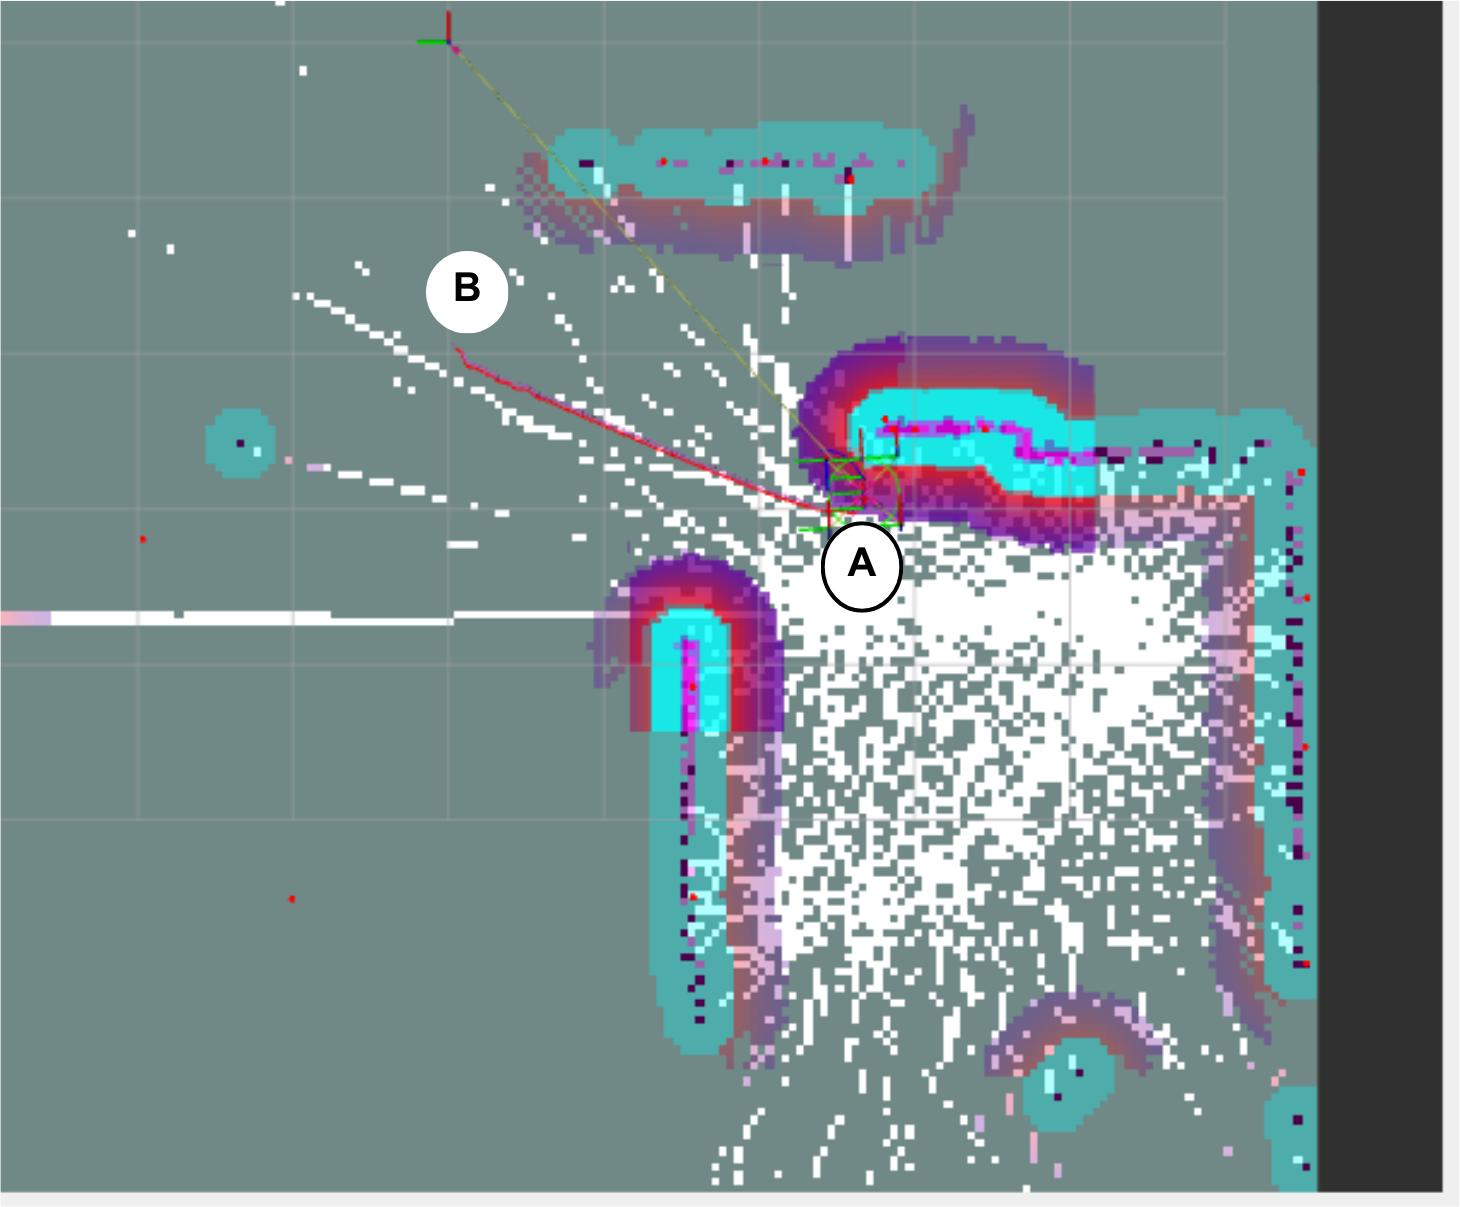
\includegraphics[scale=0.4]{trajetoria.png}
    \caption*{Fonte: Autora (2023).}
    \label{fig:trajetoriaNav2}
\end{figure}

As sub-tarefas do robô se complementam para que ele seja capaz de navegar autonomamente por um ambiente desconhecido. Foi desnecessária a implementação de um algoritmo específico para a localização do robô, como feito por \citet{navegacaoSlam:2022} com o algoritmo AMCL e por \citet{dpoom} com o aprendizado profundo reforçado. Pois, com a integração das bibliotecas Nav2 e Salm Toolbox, foi obtida essa funcionalidade de localização do robô com a dispensa de maiores incrementos.

Por fim, a implementação do Sistema Operacional de Robô (ROS) permitiu a integração entre todos os módulos e a simulação. O ROS realizou o papel crucial de intermédio entre todos os elementos do robô, permitindo que a mesma proposta possa ser utilizada além da simulação sem mudanças drásticas, como demonstrado por \citet{navegacaoSlam:2022, dpoom, lidarRGBD}.

\section{Ambiente Simulado}
O robô autônomo móvel modelado tem o objetivo de navegar de forma autônoma em um domicílio. Dito isso, o ambiente simulado foi montado para ter grande semelhança com uma residência. Para o presente trabalho é considerado como uma casa qualquer ambiente interno que contenha espaços definidos de convivência, com no mínimo um dormitório e uma cozinha. Com a ferramenta da AWS, foi possível simular um domicílio com três espaços diferentes: um dormitório, uma sala de estar e uma cozinha. Esses espaços não são divididos por paredes ou portas, possibilitando o acesso completo à casa. Cada espaço comporta elementos típicos, como cama, sofá, mesa, geladeiras e balcões. Além disso, também foram disponibilizados outros componentes para enriquecer o cenário, como produtos de academia, quadros e cabeceiras. Na Figura~\ref{fig:ambiente}, é possível visualizar o ambiente elaborado através do simulador Gazebo.

\begin{figure}[H]
    \centering
    \caption{Ambiente elaborado pela plataforma AWS}
    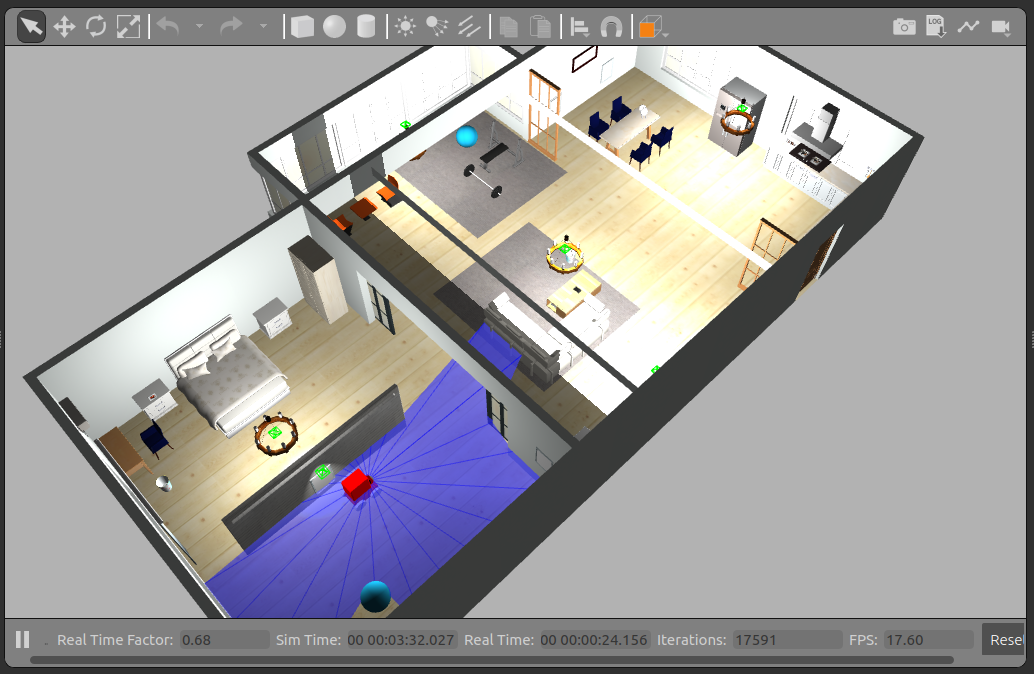
\includegraphics[scale=0.4]{ambiente.png}
    \caption*{Fonte: Autora (2023).}
    \label{fig:ambiente}
\end{figure}

\section{Resultados dos Testes}
Com o modelo proposto finalizado, foi possível validá-lo integralmente com os casos de teste elaborados e definidos no \appendixautorefname~\ref{appendix-casosTeste}. A partir dessa validação, tornou viável analisar quais os requisitos do robô, e do ambiente, foram alcançados pela implementação da solução proposta neste trabalho.

Em cada teste, foi executada a ação detalhada no caso de teste correspondente e o resultado obtido foi registrado no \appendixautorefname~\ref{appendix-resultadosTestes}. Os resultados dos casos de teste permitiram analisar quais requisitos definidos anteriormente foram alcançados com sucesso e validar o modelo completo. Os casos de teste foram elaborados conforme os requisitos levantados no início da especificação do sistema. Esses requisitos foram categorizados por prioridade no desempenho do sistema, sendo essas prioridades: i) essencial; ii) importante; iii) desejável. Com essa categorização, é possível compreender o patamar de funcionamento que o robô se encontra após desenvolvido e validado.

Os requisitos com prioridade essencial fazem parte de um conjunto de especificações que determinam os elementos fundamentais para o modelo ser funcional, sem eles o modelo não pode ser considerado um produto minimamente viável. Esses elementos tratam sobre: i) a movimentação do robô pelo ambiente sem colidir com os obstáculos presentes; ii) as mudanças frequentes que o ambiente precisa ter para representar um domicílio real com morador; iii) a verossimilhança do ambiente simulado com uma residência comum e iv) a inexistência de portas fechadas entre espaços que o robô deveria acessar, além de degraus e escadas. Diante os quatro requisitos citados, com os testes realizados, foi observado que todos eles foram alcançados.

Os requisitos com prioridade importante, são requisitos necessários para um funcionamento adequado do modelo proposto. Entretanto, a sua inexistência não limita esse funcionamento, diferente dos requisitos essenciais. Os requisitos importantes abordam a movimentação e identificação do robô. Os correspondentes testes realizados apontam que foram alcançados os dois requisitos importantes definidos previamente.

Por fim, os requisitos com prioridade desejável representam especificações que tornam ótimo o funcionamento do modelo. Caso esses requisitos não sejam atendidos, o desempenho do modelo não é afetado negativamente. Com isso, é possível serem incrementados apenas em próximas versões. Com os testes realizados, foi identificado todos os requisitos desejáveis foram alcançados.

Os casos de teste sobre a movimentação do robô e a dinamicidade do ambiente (CT01, CT02, CT03, CT04 e CT05) tiveram testes com repetições para obter o sucesso médio dos casos de teste. Os casos de teste referentes são:
\begin{enumerate}
    \item CT01 - detalha às direções possíveis que o robô é capaz de se movimentar, como demonstrado na Figura~\ref{fig:teste1CT01} com a amostra da execução de uma das repetições dos seus testes;
    \item CT02 - capacidade do robô se esquivar dos obstáculos no ambiente, como demonstrado na Figura~\ref{fig:teste1CT02}  com a amostra da execução de uma das repetições dos seus testes;
    \item CT03 - locomoção do robô em diferentes superfícies (como tapete e piso liso), como demonstrado na Figura~\ref{fig:teste1CT03}  com a amostra da execução de uma das repetições dos seus testes;
    \item CT04 - velocidade segura do robô para os seres e propriedade ao seu redor, como demonstrado na Figura~\ref{fig:teste1CT04}  com a amostra da execução de uma das repetições dos seus testes;
    \item CT05 - capacidade de alterar a posição dos elementos da simulação, como demonstrado na Figura~\ref{fig:teste1CT05}  com a amostra da execução de uma das repetições dos seus testes.
\end{enumerate}

\begin{figure}[H]
    \centering
    \caption{Captura da primeira repetição CT01}
    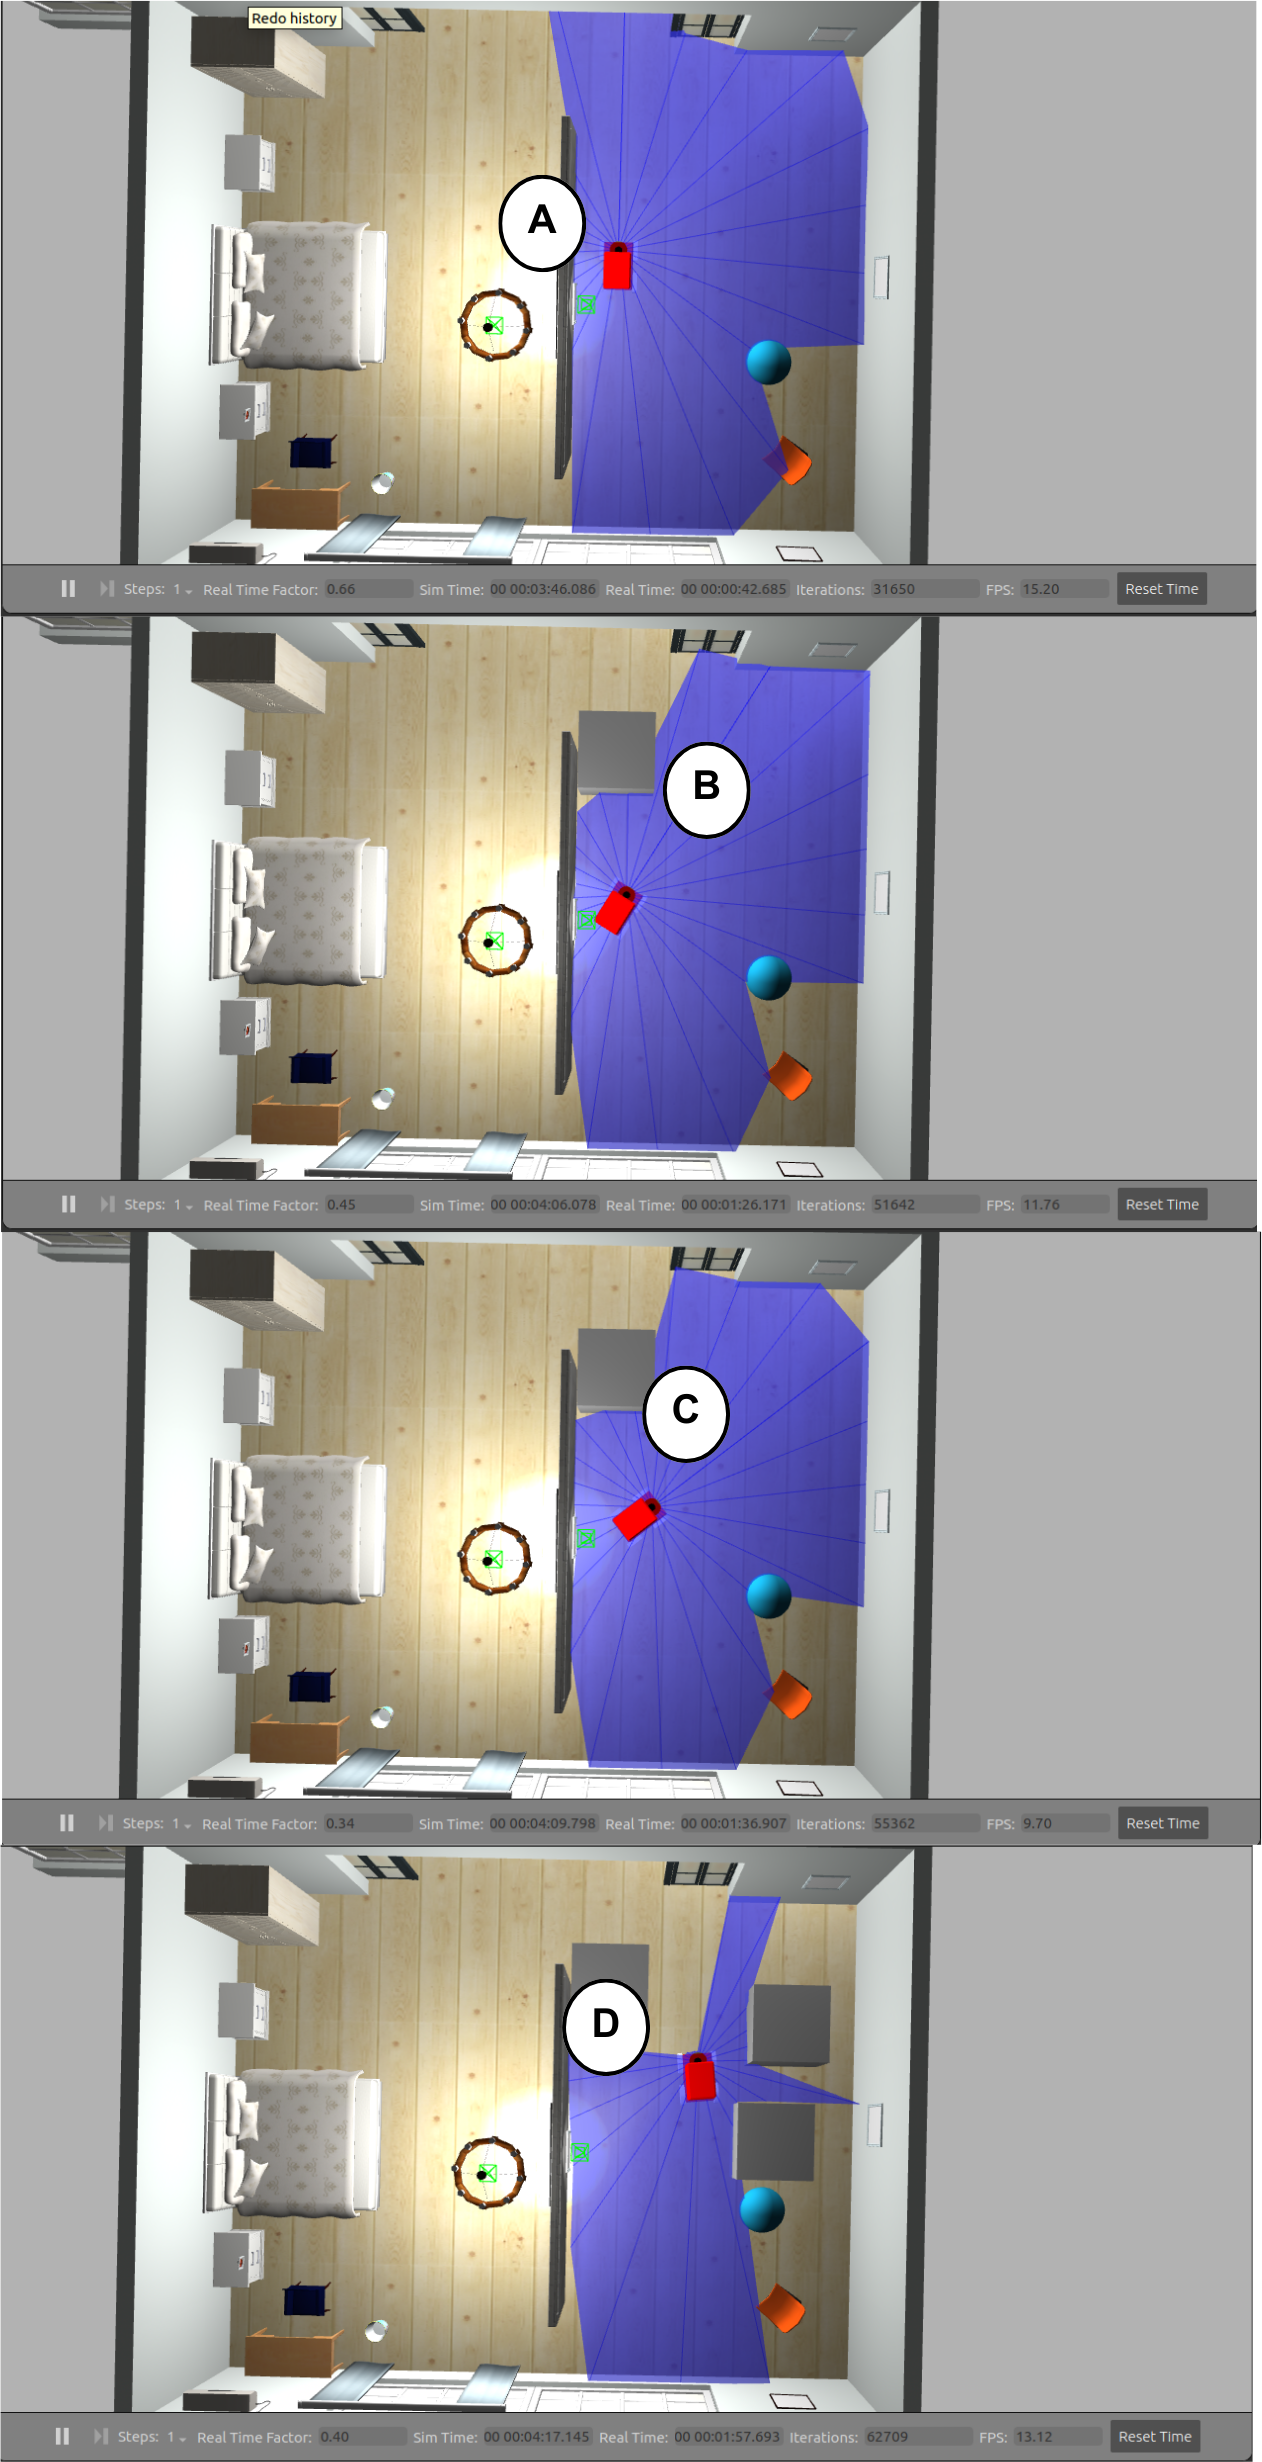
\includegraphics[scale=0.35]{ct01_1.png}
    \caption*{Fonte: Autora (2023).}
    \label{fig:teste1CT01}
\end{figure}

\begin{figure}[H]
    \centering
    \caption{Captura da primeira repetição CT02}
    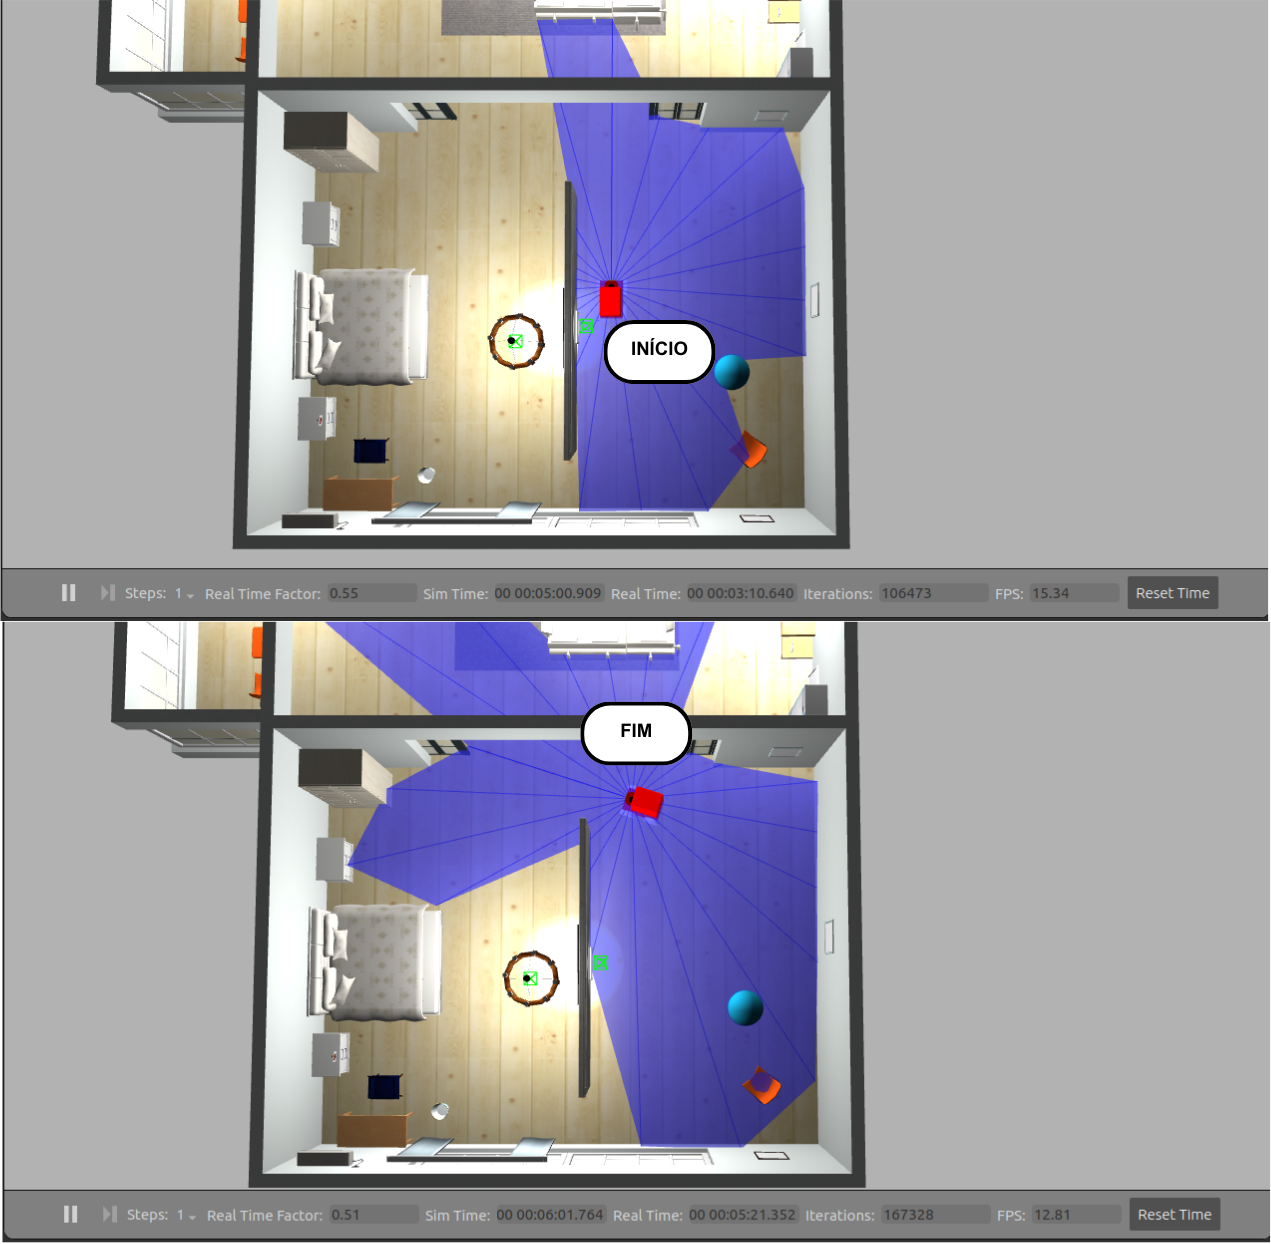
\includegraphics[scale=0.3]{ct02_1.png}
    \caption*{Fonte: Autora (2023).}
    \label{fig:teste1CT02}
\end{figure}

\begin{figure}[H]
    \centering
    \caption{Captura da primeira repetição CT03}
    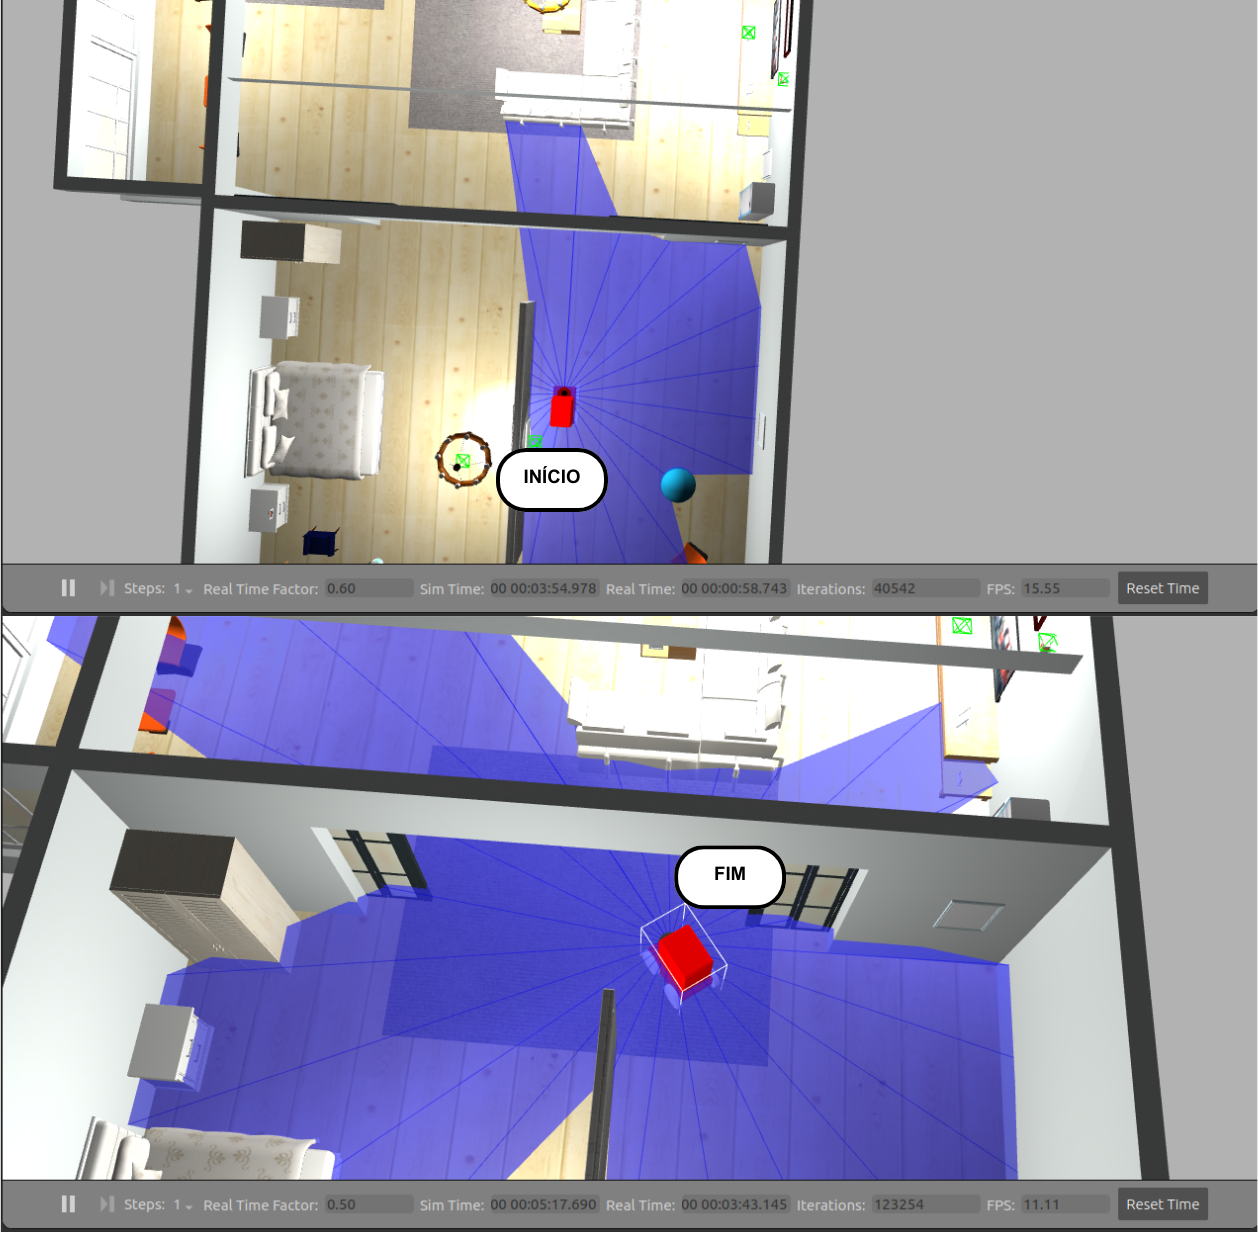
\includegraphics[scale=0.3]{ct03_1.png}
    \caption*{Fonte: Autora (2023).}
    \label{fig:teste1CT03}
\end{figure}

\begin{figure}[H]
    \centering
    \caption{Captura da primeira repetição CT04}
    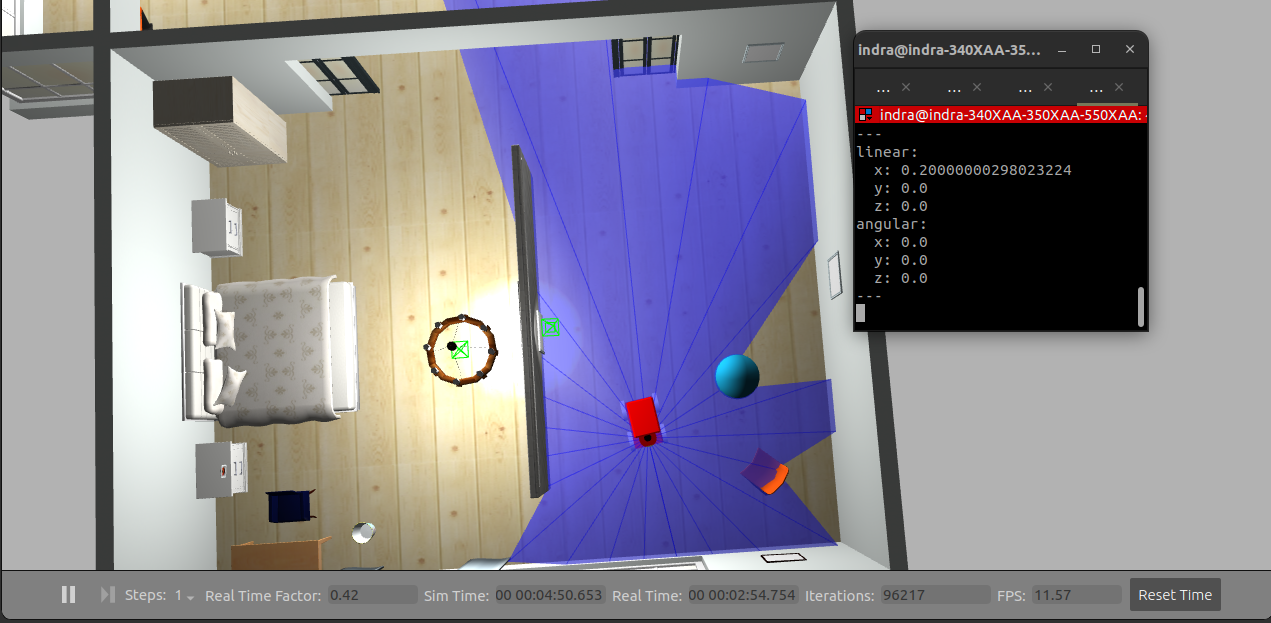
\includegraphics[scale=0.33]{ct04_1.png}
    \caption*{Fonte: Autora (2023).}
    \label{fig:teste1CT04}
\end{figure}

\begin{figure}[H]
    \centering
    \caption{Captura da primeira repetição CT05}
    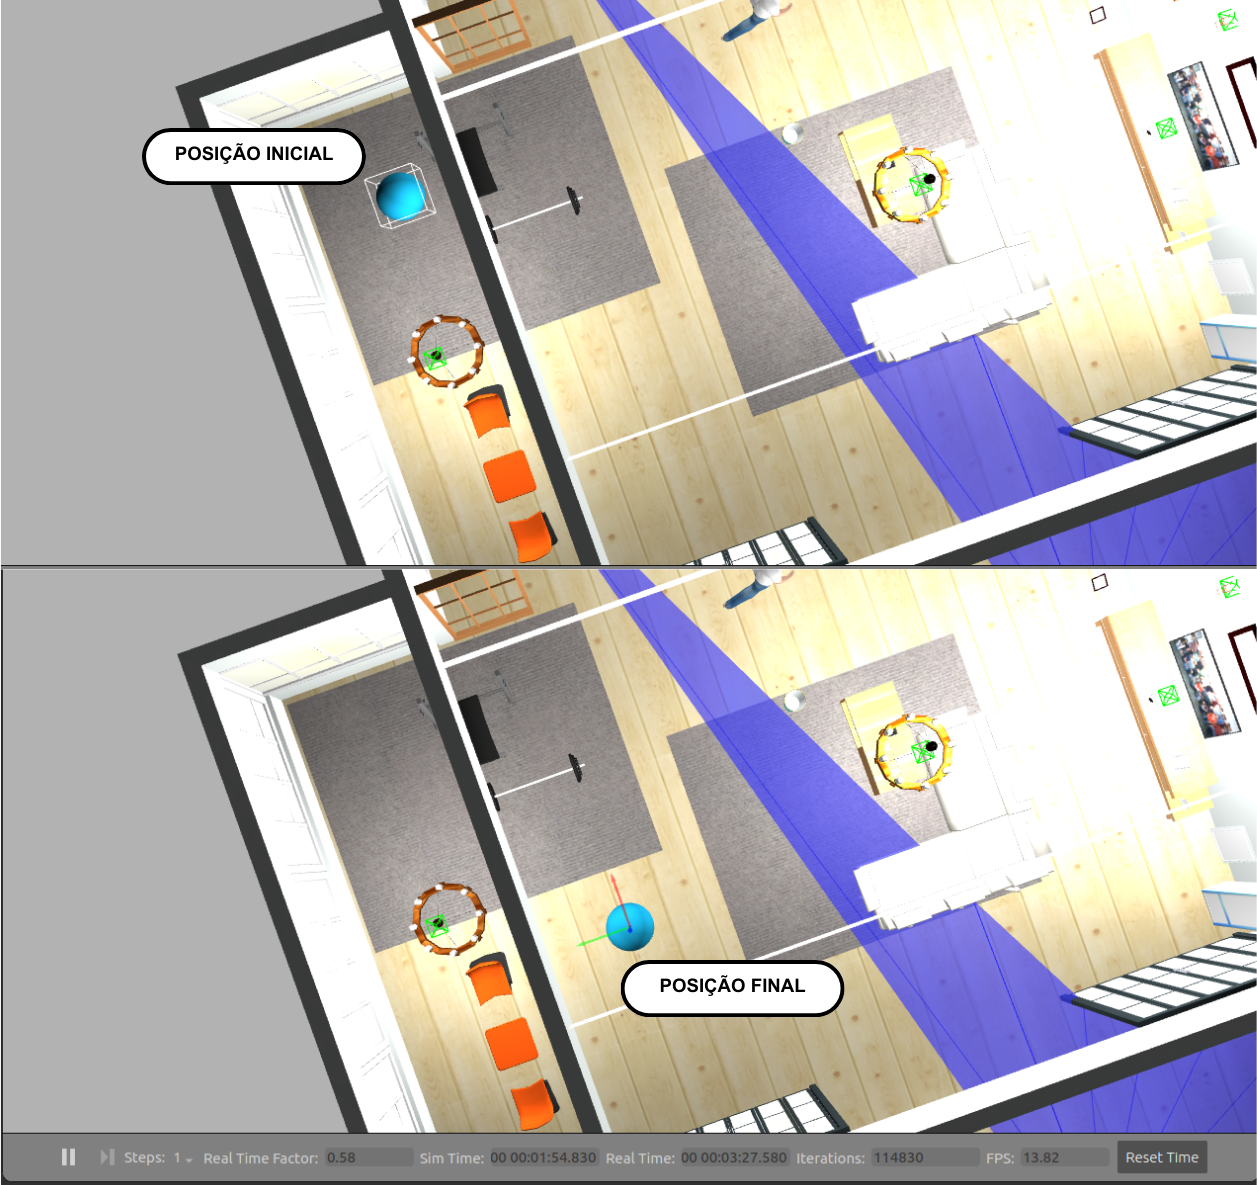
\includegraphics[scale=0.4]{ct05_1.png}
    \caption*{Fonte: Autora (2023).}
    \label{fig:teste1CT05}
\end{figure}

Dito isso, com as cinco repetições para os testes referentes aos casos de teste citados, foram obtidos apenas dois casos de teste com uma porcentagem de 80\% de sucesso. Dentre as 25 repetições de cinco casos de teste diferentes, os cenários CT01 e CT02  apresentaram uma taxa de sucesso menor que 100\%  (Figura~\ref{fig:sucessoTestes}).

\begin{figure}[h]
    \centering
    \caption{Resultados dos testes com repetições}
    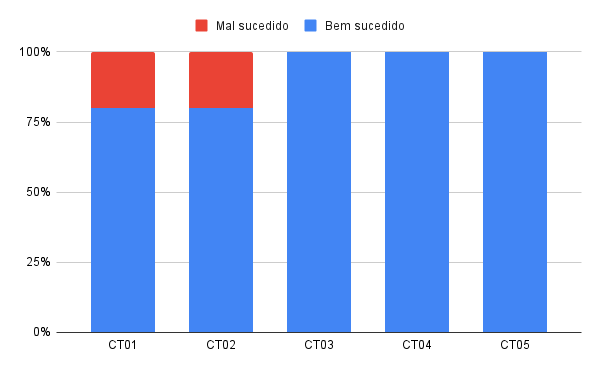
\includegraphics[scale=0.65]{sucessoTestes.png}
    \caption*{Fonte: Autora (2023).}
    \label{fig:sucessoTestes}
\end{figure}

Os casos de teste que obtiveram uma taxa de 80\% de sucesso correspondiam a capacidade do movimento do robô em todos os eixos e na sua locomoção pelo ambiente sem colidir com obstáculos. Os testes para o primeiro caso de teste (CT01) apresentaram uma falha de 20\%, ocasionada pelo mau posicionamento dos obstáculos (Figura~\ref{fig:erroCT01}).

\begin{figure}[p]
    \centering
    \caption{Captura da repetição do CT01 mal-sucedida }
    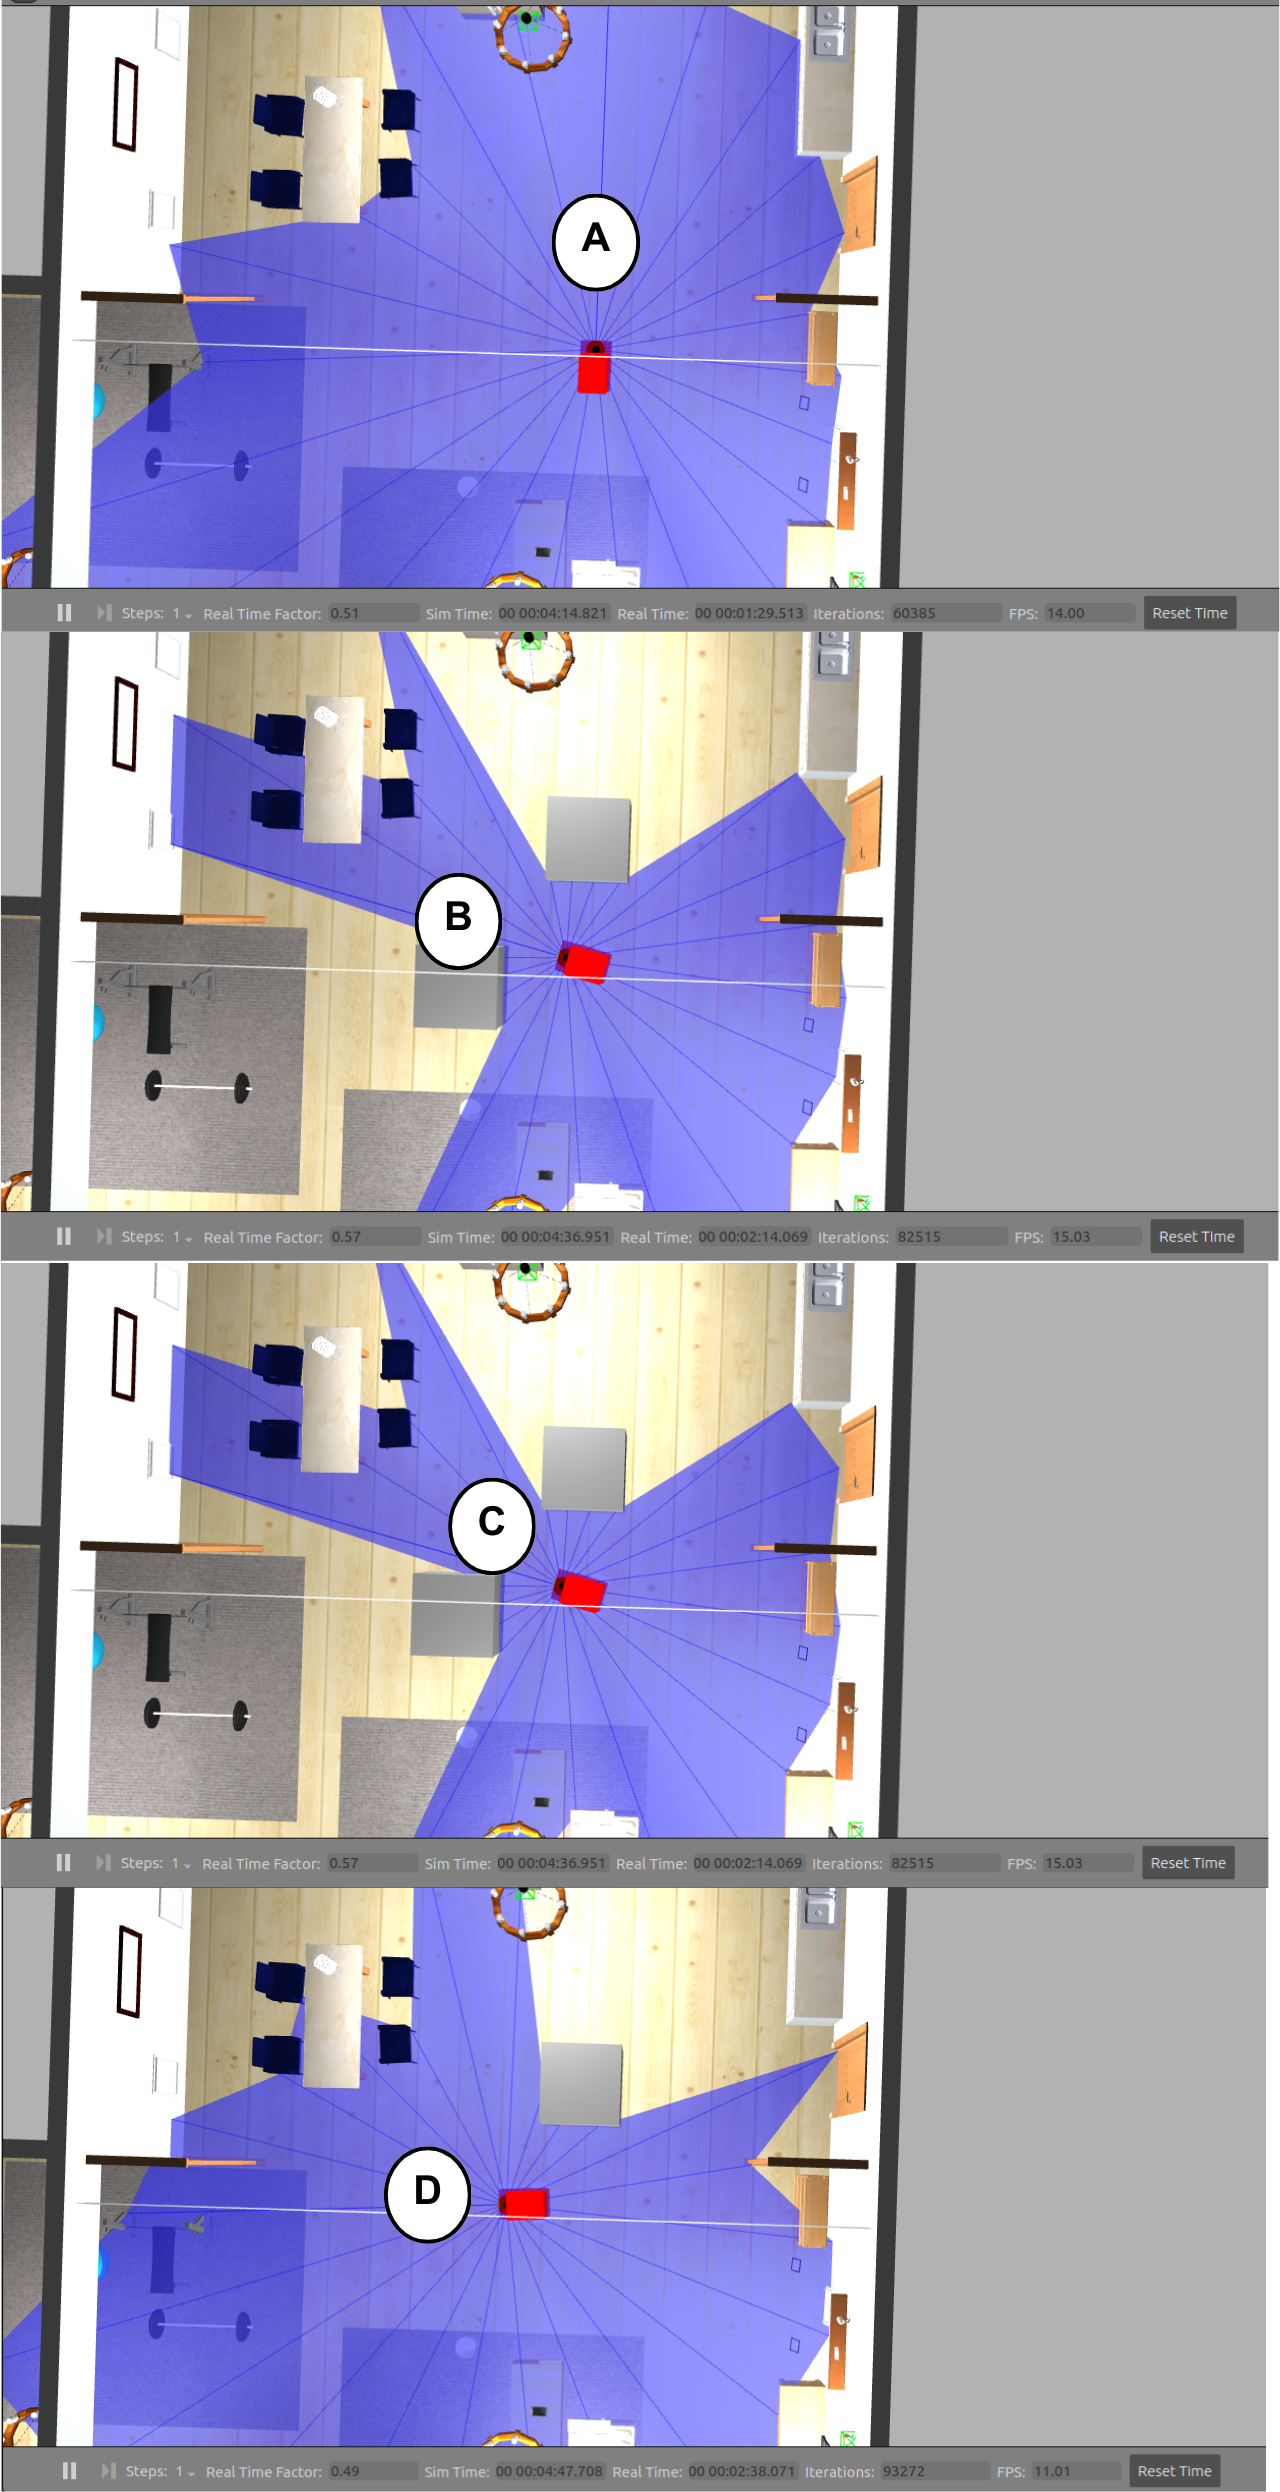
\includegraphics[scale=0.3]{ct01_4.png}
    \caption*{Fonte: Autora (2023).}
    \label{fig:erroCT01}
\end{figure}

O teste mal-sucedido para o segundo caso de teste (CT02), teve esse resultado devido ao local estreito na trajetória do robô (Figura~\ref{fig:erroCT02}). Para momentos no qual o robô se encontra sem opção, \citet{lidarRGBD} implementaram um estado de recuperação para que o robô possa retornar à sua navegação, podendo ser vantajoso em situações como a encontrada nesse teste com resultado negativo. Por ser uma porcentagem de falha mínima perante todos os sucessos, esses testes mal-sucedidos não impactam negativamente na navegação autônoma do robô. 

\begin{figure}[H]
    \centering
    \caption{Captura da repetição CT02 mal-sucedida}
    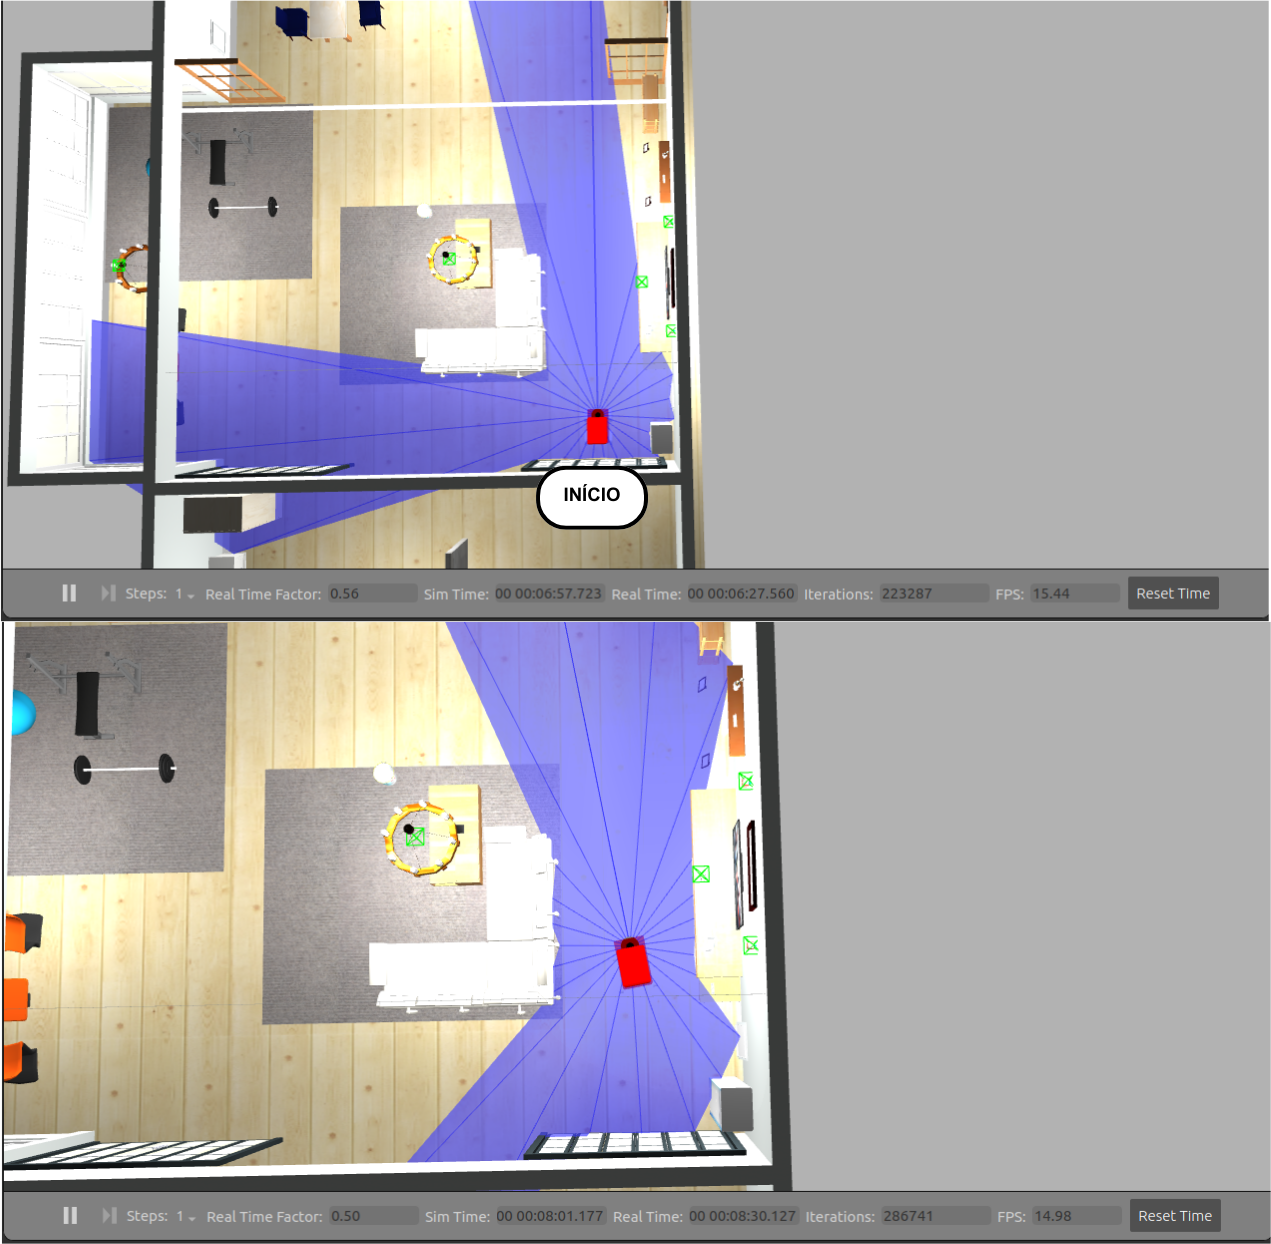
\includegraphics[scale=0.3]{ct02_4.png}
    \caption*{Fonte: Autora (2023).}
    \label{fig:erroCT02}
\end{figure}

Por fim, a simulação no programa Gazebo proporcionou a verificação da implementação das funcionalidades. Com isso, ao longo do desenvolvimento, foi possível analisar as integrações e realizar as mudanças necessárias para a melhoria dos componentes. Tal facilidade na validação do comportamento do robô pela simulação também é aproveitada por \citet{navegacaoSlam:2022, dpoom, lidarRGBD}. 

\section{Destaques do AtmosBot}
A implementação completa do modelo proposto permite uma comparação dos seus resultados obtidos e dos trabalhos correlatos. Na Tabela~\ref{tab:comparacaoResultados} estão expostos os resultados obtidos na navegação autônoma do AtmosBot e os trabalhos correlatos explicados no \chapterautorefname~\ref{cap-trabalhos-relacionados}. A tabela separa a navegação nas suas principais atividades, enfatizando as tecnologias implementadas e suas consequências.

\begin{table}[h]
    \centering
    \caption{Comparação dos resultados do AtmosBot com trabalhos correlatos}
    \label{tab:comparacaoResultados}
    \resizebox{\textwidth}{!}{%
    \begin{tabular}{p{3cm}|p{3cm}|p{3cm}|p{3cm}}
        & \multicolumn{1}{p{3cm}|}{\textbf{Percepção}} & \multicolumn{1}{p{3cm}|}{\textbf{Localização}}                    & \multicolumn{1}{p{3cm}}{\textbf{Mapeamento}}   \\ \hline 
\textbf{AtmosBot} &
Sensor LiDaR: menor custo de processamento e tecnologia mais relevante &
Biblioteca Nav2 + Slam Toolbox: implementação em mais alto nível &
Slam + navegação: abordagem mais relevante e menor divergência no mapeamento \\ \hline
\textbf{Robô TurtleBot3 Burger de \citet{turtleBot3Burger:2021}} &
sensor LiDaR: integração mais relevante com SLAM e ROS &
AMCL: implementação com pacotes do ROS e menos colisões &
Slam com mapa criado antes da navegação: robô controlado remotamente e divergência com mundo real \\ \hline
\textbf{Robô DPoom de \citet{dpoom}} & câmera RGB-D: menor custo financeiro    & Mapas 3D + câmera RGB-D: sem implementação de outros pacotes & Slam 3D: criação de mapas mais detalhados \\ \hline
\textbf{Robô com LiDaR e RGB-D \citet{lidarRGBD}} &
sensor LiDaR e câmera RGB-D: percepção 3D do ambiente &
AMCL: implementação extra com pacotes do ROS &
Slam 2D e mapa estático: robô controlado remotamente
\end{tabular}%
    }
    \caption*{Fonte: Autora (2023).}
\end{table}

\newpage

Como pode ser observado na Tabela~\ref{tab:comparacaoResultados}, um dos principais destaques do AtmosBot é a implementação de tecnologias relevantes para a percepção e mapeamento do ambiente, obtendo um menor custo de processamento e divergência do mundo real. Além disso, foi possível obter a localização do robô com bibliotecas integradas ao ROS, sem a necessidade de implementar um algoritmo específico em baixo nível.